\chapter{Singularity Analysis}
\label{chap:3}


In this chapter I will discuss my stylistic choices of \textsf{sapthesis}.
I will show the page layout geometry and I will describe the page style. \cite{Shirazi2014}


\begin{figure}[!h]
    \centering
    

\tikzset{every picture/.style={line width=0.75pt}} %set default line width to 0.75pt        

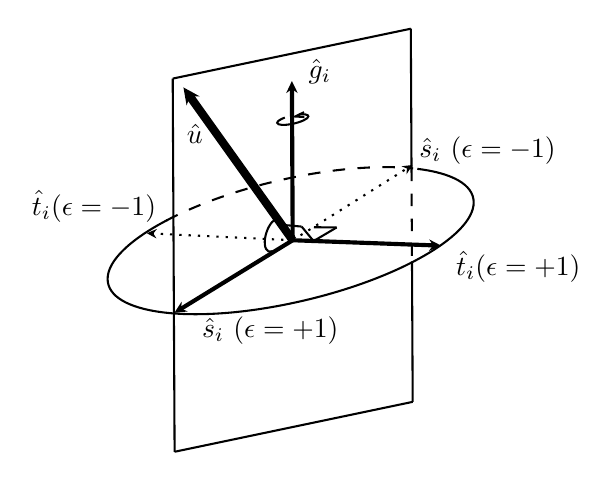
\begin{tikzpicture}[x=0.5pt,y=0.5pt,yscale=-1,xscale=1]
%uncomment if require: \path (0,348); %set diagram left start at 0, and has height of 348

%Straight Lines [id:da7916208743434348] 
\draw [line width=1.5]    (325.78,157.42) -- (243.69,207.79) ;
\draw [shift={(240.28,209.89)}, rotate = 328.47] [fill={rgb, 255:red, 0; green, 0; blue, 0 }  ][line width=0.08]  [draw opacity=0] (8.75,-4.2) -- (0,0) -- (8.75,4.2) -- (5.81,0) -- cycle    ;
%Straight Lines [id:da6063053587743079] 
\draw [line width=1.5]    (325.78,157.42) -- (429.04,161.18) ;
\draw [shift={(433.04,161.33)}, rotate = 182.09] [fill={rgb, 255:red, 0; green, 0; blue, 0 }  ][line width=0.08]  [draw opacity=0] (8.75,-4.2) -- (0,0) -- (8.75,4.2) -- (5.81,0) -- cycle    ;
%Straight Lines [id:da8584098766750565] 
\draw [line width=1.5]    (325.78,157.42) -- (325.22,46.36) ;
\draw [shift={(325.2,42.36)}, rotate = 449.71] [fill={rgb, 255:red, 0; green, 0; blue, 0 }  ][line width=0.08]  [draw opacity=0] (8.75,-4.2) -- (0,0) -- (8.75,4.2) -- (5.81,0) -- cycle    ;
%Straight Lines [id:da36750414352491156] 
\draw  [dash pattern={on 0.84pt off 2.51pt}]  (325.78,157.42) -- (409.76,104.66) ;
\draw [shift={(412.3,103.06)}, rotate = 507.86] [fill={rgb, 255:red, 0; green, 0; blue, 0 }  ][line width=0.08]  [draw opacity=0] (7.14,-3.43) -- (0,0) -- (7.14,3.43) -- (4.74,0) -- cycle    ;
%Straight Lines [id:da051548852230852926] 
\draw  [dash pattern={on 0.84pt off 2.51pt}]  (325.78,157.42) -- (223.36,152.49) ;
\draw [shift={(220.36,152.35)}, rotate = 362.75] [fill={rgb, 255:red, 0; green, 0; blue, 0 }  ][line width=0.08]  [draw opacity=0] (7.14,-3.43) -- (0,0) -- (7.14,3.43) -- (4.74,0) -- cycle    ;
%Straight Lines [id:da17659245242461763] 
\draw [line width=3]    (325.78,157.42) -- (276.96,89.13) -- (250.31,51.86) ;
\draw [shift={(246.82,46.98)}, rotate = 414.43] [fill={rgb, 255:red, 0; green, 0; blue, 0 }  ][line width=0.08]  [draw opacity=0] (11.97,-5.75) -- (0,0) -- (11.97,5.75) -- (7.95,0) -- cycle    ;
%Straight Lines [id:da48871347567863976] 
\draw    (341.17,148.01) -- (357.58,148.17) ;
%Straight Lines [id:da5947811121524507] 
\draw    (340.86,158.03) -- (357.58,148.17) ;
%Straight Lines [id:da18808003722282884] 
\draw    (318.62,146.33) -- (332.25,147.55) ;
%Straight Lines [id:da3929565984820087] 
\draw    (332.25,147.55) -- (340.86,158.03) ;
%Shape: Arc [id:dp1302171161481871] 
\draw  [draw opacity=0] (311.27,165.16) .. controls (311.04,165.28) and (310.81,165.38) .. (310.58,165.46) .. controls (306.98,166.74) and (304.84,162.5) .. (305.8,156) .. controls (306.72,149.85) and (310.07,143.88) .. (313.48,142.17) -- (312.33,153.69) -- cycle ; \draw   (311.27,165.16) .. controls (311.04,165.28) and (310.81,165.38) .. (310.58,165.46) .. controls (306.98,166.74) and (304.84,162.5) .. (305.8,156) .. controls (306.72,149.85) and (310.07,143.88) .. (313.48,142.17) ;
%Shape: Arc [id:dp4658593680079681] 
\draw  [draw opacity=0] (415.85,105.83) .. controls (440.9,108.83) and (456.52,117.16) .. (456.59,130) .. controls (456.72,155.04) and (397.59,187.75) .. (324.53,203.07) .. controls (251.47,218.39) and (192.14,210.5) .. (192.01,185.46) .. controls (191.94,172.1) and (208.74,156.56) .. (235.52,142.64) -- (324.3,157.73) -- cycle ; \draw   (415.85,105.83) .. controls (440.9,108.83) and (456.52,117.16) .. (456.59,130) .. controls (456.72,155.04) and (397.59,187.75) .. (324.53,203.07) .. controls (251.47,218.39) and (192.14,210.5) .. (192.01,185.46) .. controls (191.94,172.1) and (208.74,156.56) .. (235.52,142.64) ;
%Shape: Arc [id:dp7085048189876144] 
\draw  [draw opacity=0][dash pattern={on 4.5pt off 4.5pt}] (234.57,143.14) .. controls (258.09,130.76) and (289.52,119.63) .. (324.07,112.39) .. controls (358.2,105.23) and (389.34,103.14) .. (412.84,105.5) -- (324.3,157.73) -- cycle ; \draw  [dash pattern={on 4.5pt off 4.5pt}] (234.57,143.14) .. controls (258.09,130.76) and (289.52,119.63) .. (324.07,112.39) .. controls (358.2,105.23) and (389.34,103.14) .. (412.84,105.5) ;
%Straight Lines [id:da5865544576762574] 
\draw    (411.14,4.55) -- (411.65,105.77) ;
%Straight Lines [id:da7590207701341669] 
\draw    (239.07,40.6) -- (240.43,310.29) ;
%Straight Lines [id:da790374687044014] 
\draw    (239.07,40.6) -- (411.14,4.55) ;
%Straight Lines [id:da17494293181301823] 
\draw    (240.43,310.29) -- (412.5,274.23) ;
%Straight Lines [id:da5701402858596814] 
\draw    (411.99,172.73) -- (412.5,274.23) ;
%Straight Lines [id:da2349258321762262] 
\draw  [dash pattern={on 4.5pt off 4.5pt}]  (411.65,105.77) -- (411.99,172.73) ;
%Shape: Arc [id:dp4799622522622564] 
\draw  [draw opacity=0] (330.58,66.45) .. controls (334.42,66.13) and (337.09,66.63) .. (337.1,67.85) .. controls (337.1,69.54) and (332.07,71.96) .. (325.85,73.26) .. controls (319.63,74.57) and (314.58,74.26) .. (314.58,72.57) .. controls (314.57,71.45) and (316.78,70.01) .. (320.09,68.78) -- (325.84,70.21) -- cycle ; \draw   (330.58,66.45) .. controls (334.42,66.13) and (337.09,66.63) .. (337.1,67.85) .. controls (337.1,69.54) and (332.07,71.96) .. (325.85,73.26) .. controls (319.63,74.57) and (314.58,74.26) .. (314.58,72.57) .. controls (314.57,71.45) and (316.78,70.01) .. (320.09,68.78) ;
\draw   (333.97,64.87) -- (327.59,67.99) -- (334.21,68.38) ;

% Text Node
\draw (441.66,162.98) node [anchor=north west][inner sep=0.75pt]    {$\hat{t}_{i}( \epsilon =+1)$};
% Text Node
\draw (258,210.4) node [anchor=north west][inner sep=0.75pt]    {$\hat{s}_{i} \ ( \epsilon =+1)$};
% Text Node
\draw (415,80.4) node [anchor=north west][inner sep=0.75pt]    {$\hat{s}_{i} \ ( \epsilon =-1)$};
% Text Node
\draw (135,119.4) node [anchor=north west][inner sep=0.75pt]    {$\hat{t}_{i}( \epsilon =-1)$};
% Text Node
\draw (247,71.4) node [anchor=north west][inner sep=0.75pt]    {$\hat{u}$};
% Text Node
\draw (335,24.4) node [anchor=north west][inner sep=0.75pt]    {$\hat{g}_{i}$};
\end{tikzpicture}

    \caption{Vector representation at singular gimble state}
    \label{fig:tikCMG}
\end{figure}

\begin{figure}[h]
\centering
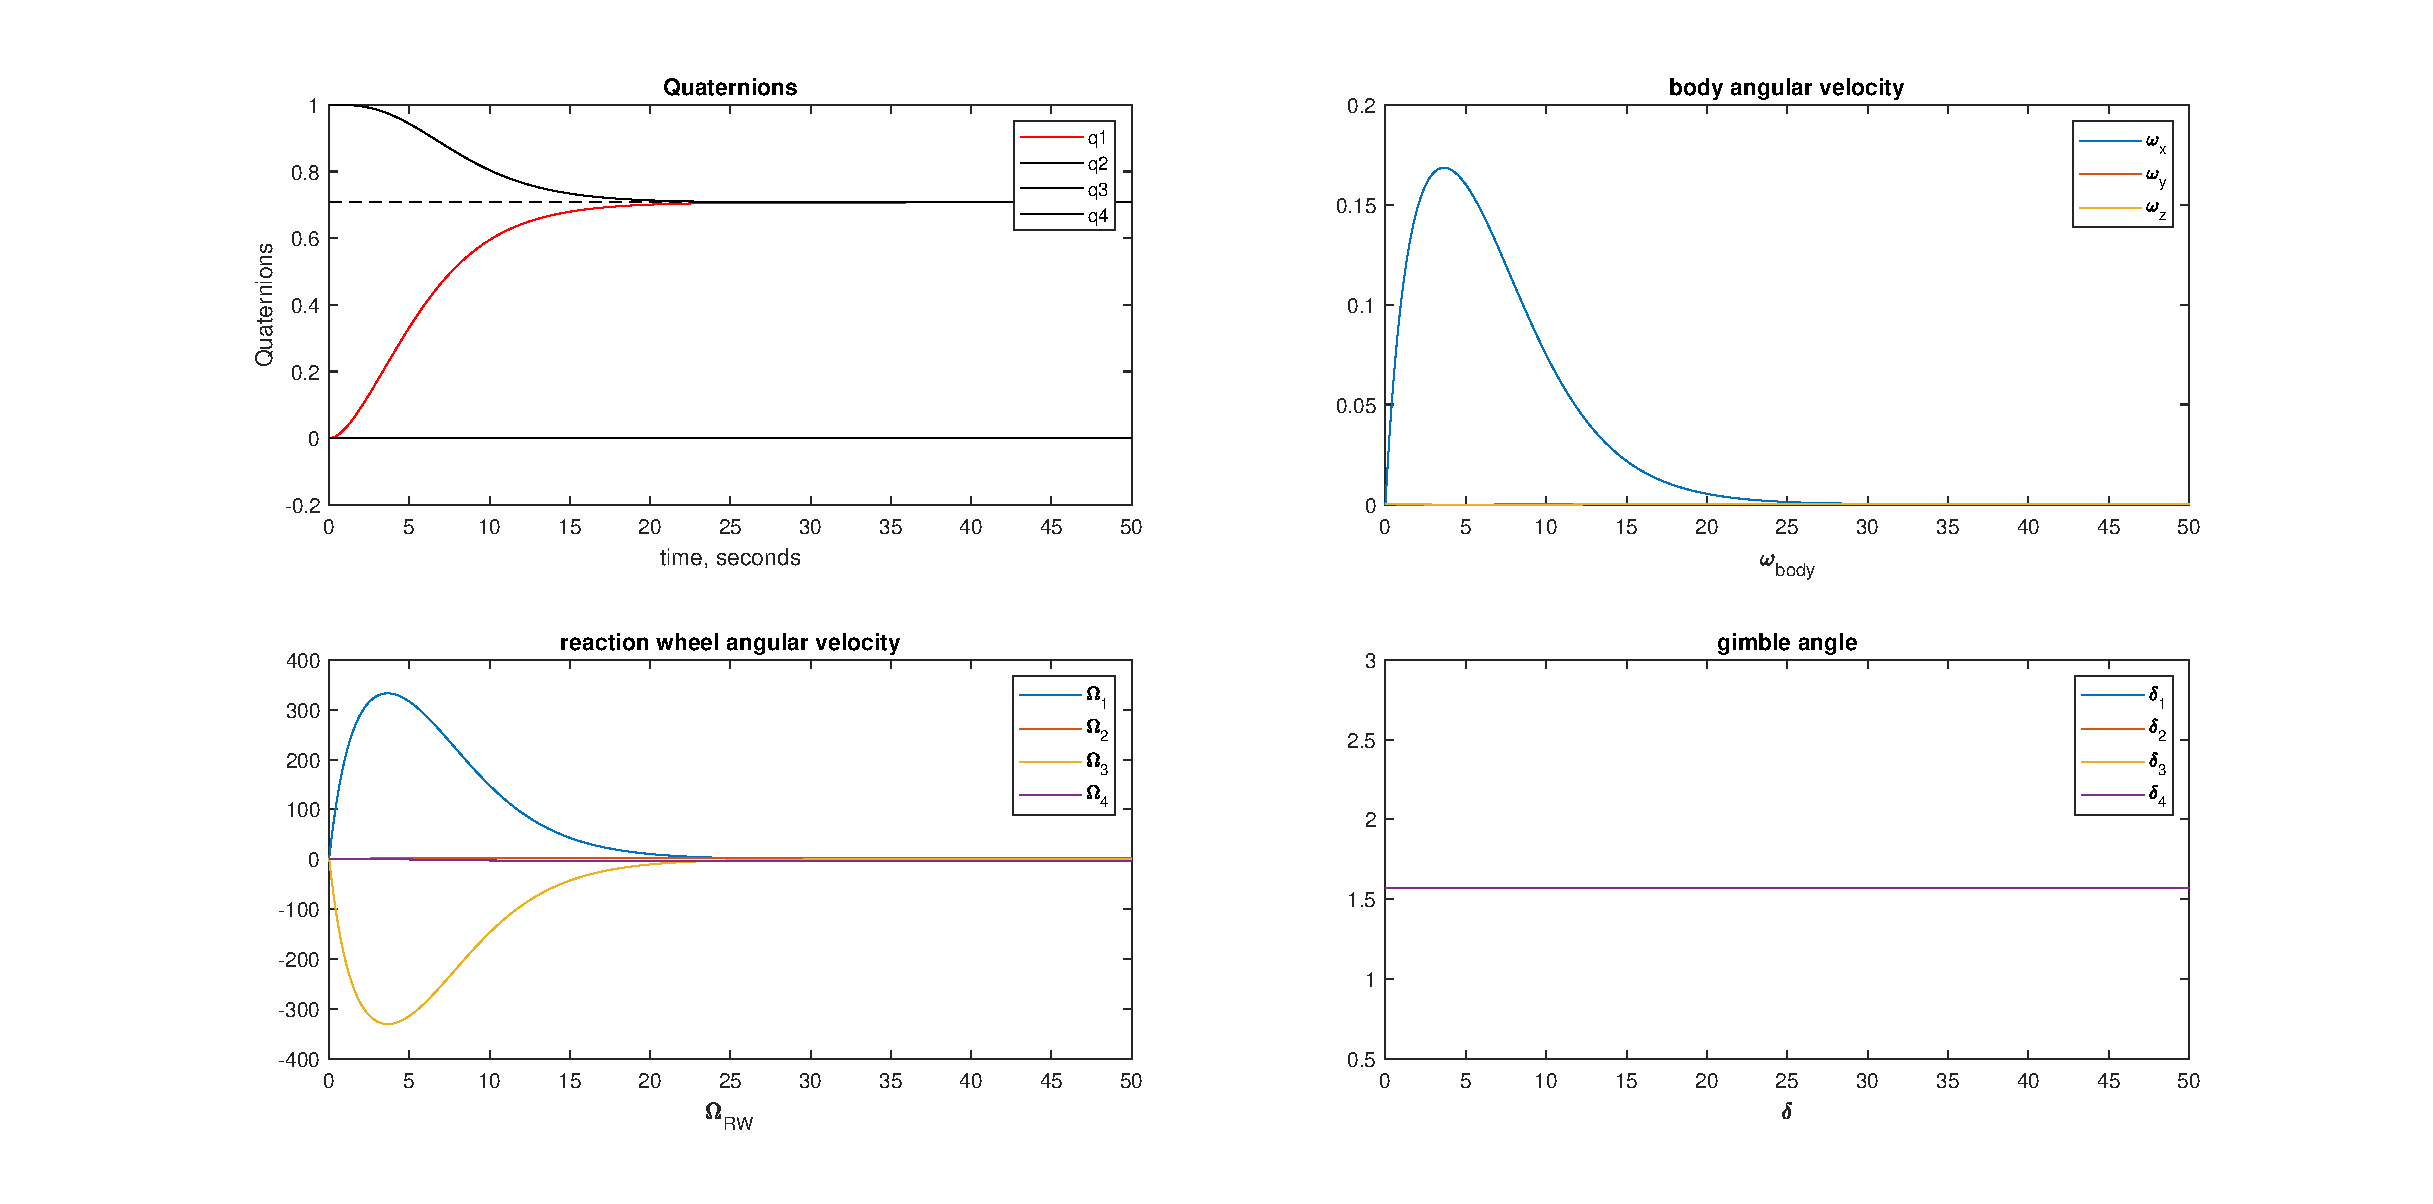
\includegraphics[scale=0.5]{figures/fig4.eps}
\end{figure}

\section{Page layout}

The page is fixed at the dimensions of an A4 paper, therefore you have to print your thesis on A4 paper to obtain the best results. The font dimension is fixed at 11\, pt. The text column and the margins are chosen to fill to the best an A4 paper while keeping a reasonable line length (396\, pt) for a good readability. The text height and the text width are in golden ratio (\textasciitilde 1.6180) as well as the outer and inner margins in a two-side document after binding margin removal. Also the top margin (excluding the header) and bottom margin are in the golden ratio. In Fig.~\ref{layout} a sketch of the \textsf{sapthesis} page layout is shown. \acrlong{vscmg}

\begin{figure}[h]
\centering
\setlength{\unitlength}{0.27mm}
\begin{picture}(420,297)(-210,0)
\polyline(-210,0)(210,0)(210,297)(-210,297)(-210,0)
\Line(0,0)(0,297)
\put(27.05,37.4){\polygon(0,0)(139.2,0)(139.2,223.8)(0,223.8)}
\put(-27.05,37.4){\polygon(0,0)(-139.2,0)(-139.2,223.8)(0,223.8)}
\put(27.05,268.16){\polygon(0,0)(139.2,0)(139.2,4.22)(0,4.22)}
\put(-27.05,268.16){\polygon(0,0)(-139.2,0)(-139.2,4.22)(0,4.22)}
\end{picture}
\caption{Page layout scheme of \textsf{sapthesis class} using a zero binding margin.}
\label{layout}
\end{figure}


\section{Page style}

The captions have a smaller font respect to the text and the label is in boldface. The appearance of the margin notes has been improved.
They have the same font dimension of the footnotes and are typed in italics.
Moreover I defined a new command to typeset margin note aligned to the left on the right page and vice versa on the left page.
Notice that if a binding margin greater than 1.5\, cm is used, the dimensions of the margin notes become too small and very ugly.
Do not use them in this case.

The mathematical objects, figures and tables are numbered within the chapters (e.g. 1.1, 1.2,\ldots for the first chapter, 2.1, 2.2 for the second one and so on\ldots). See for example the number of this simple equation
\begin{equation}
x_{1,2}=\frac{-b\pm\sqrt{b^2-4ac}}{2a}
\end{equation}


The title page is automatically composed when the \texttt{\bs maketitle} command is given.
The parameters needed for the title page, author, title, etc\ldots , are supplied by dedicated commands explained in the next section.
Two copies of the university logo in \texttt{pdf} format, one for color printing and the other one for black and white printing, are supplied in the \textsf{sapthesis} package. They are shown in Fig.~\ref{fig:largenenough}.

\begin{figure}
\centering
\includegraphics[width=0.7\textwidth]{sapienza-MLred-pos}\\[3ex]
\includegraphics[width=0.7\textwidth]{sapienza-MLblack-pos}
\caption{Logo of the Sapienza -- University of Rome.}
\label{fig:largenenough}
\end{figure}



\section{About figures and tables}

As regards the image formats, please use vector images as much as possible! Use jpg images only for photographs! pdf\LaTeX\ supports the pdf, jpg and png formats.

A very simple table is show in Tab.~\ref{tab:letters}. Remember to typeset
always the table caption above the table. Do not use vertical lines.

\begin{table}
\caption{This is a simple table.}
\label{tab:letters}
\centering
\begin{tabular}{lcc}
\toprule
Letter & Test & Test \\
\midrule
A & C & E \\
B & D & F \\
\bottomrule
\end{tabular}
\end{table}


\section{A section}

In this manual you can skip the gray text because it is just dummy text.



\section{Another section}

In this manual you can skip the gray text because it is just dummy text.

